\chapter{Supplementary Local Explanations}
\label{app:local_explanations}

This appendix presents the representative \gls{lime} explanations referenced in Chapter~\ref{chap:xai_results}. Each panel reports seed-averaged local surrogate rules for the selected prediction outcomes. The figures are descriptive examples of fitted-model behaviour and should be read with the case-selection and seed-stability analyses in the main chapter.

\begin{sidewaysfigure}[p]
    \centering
    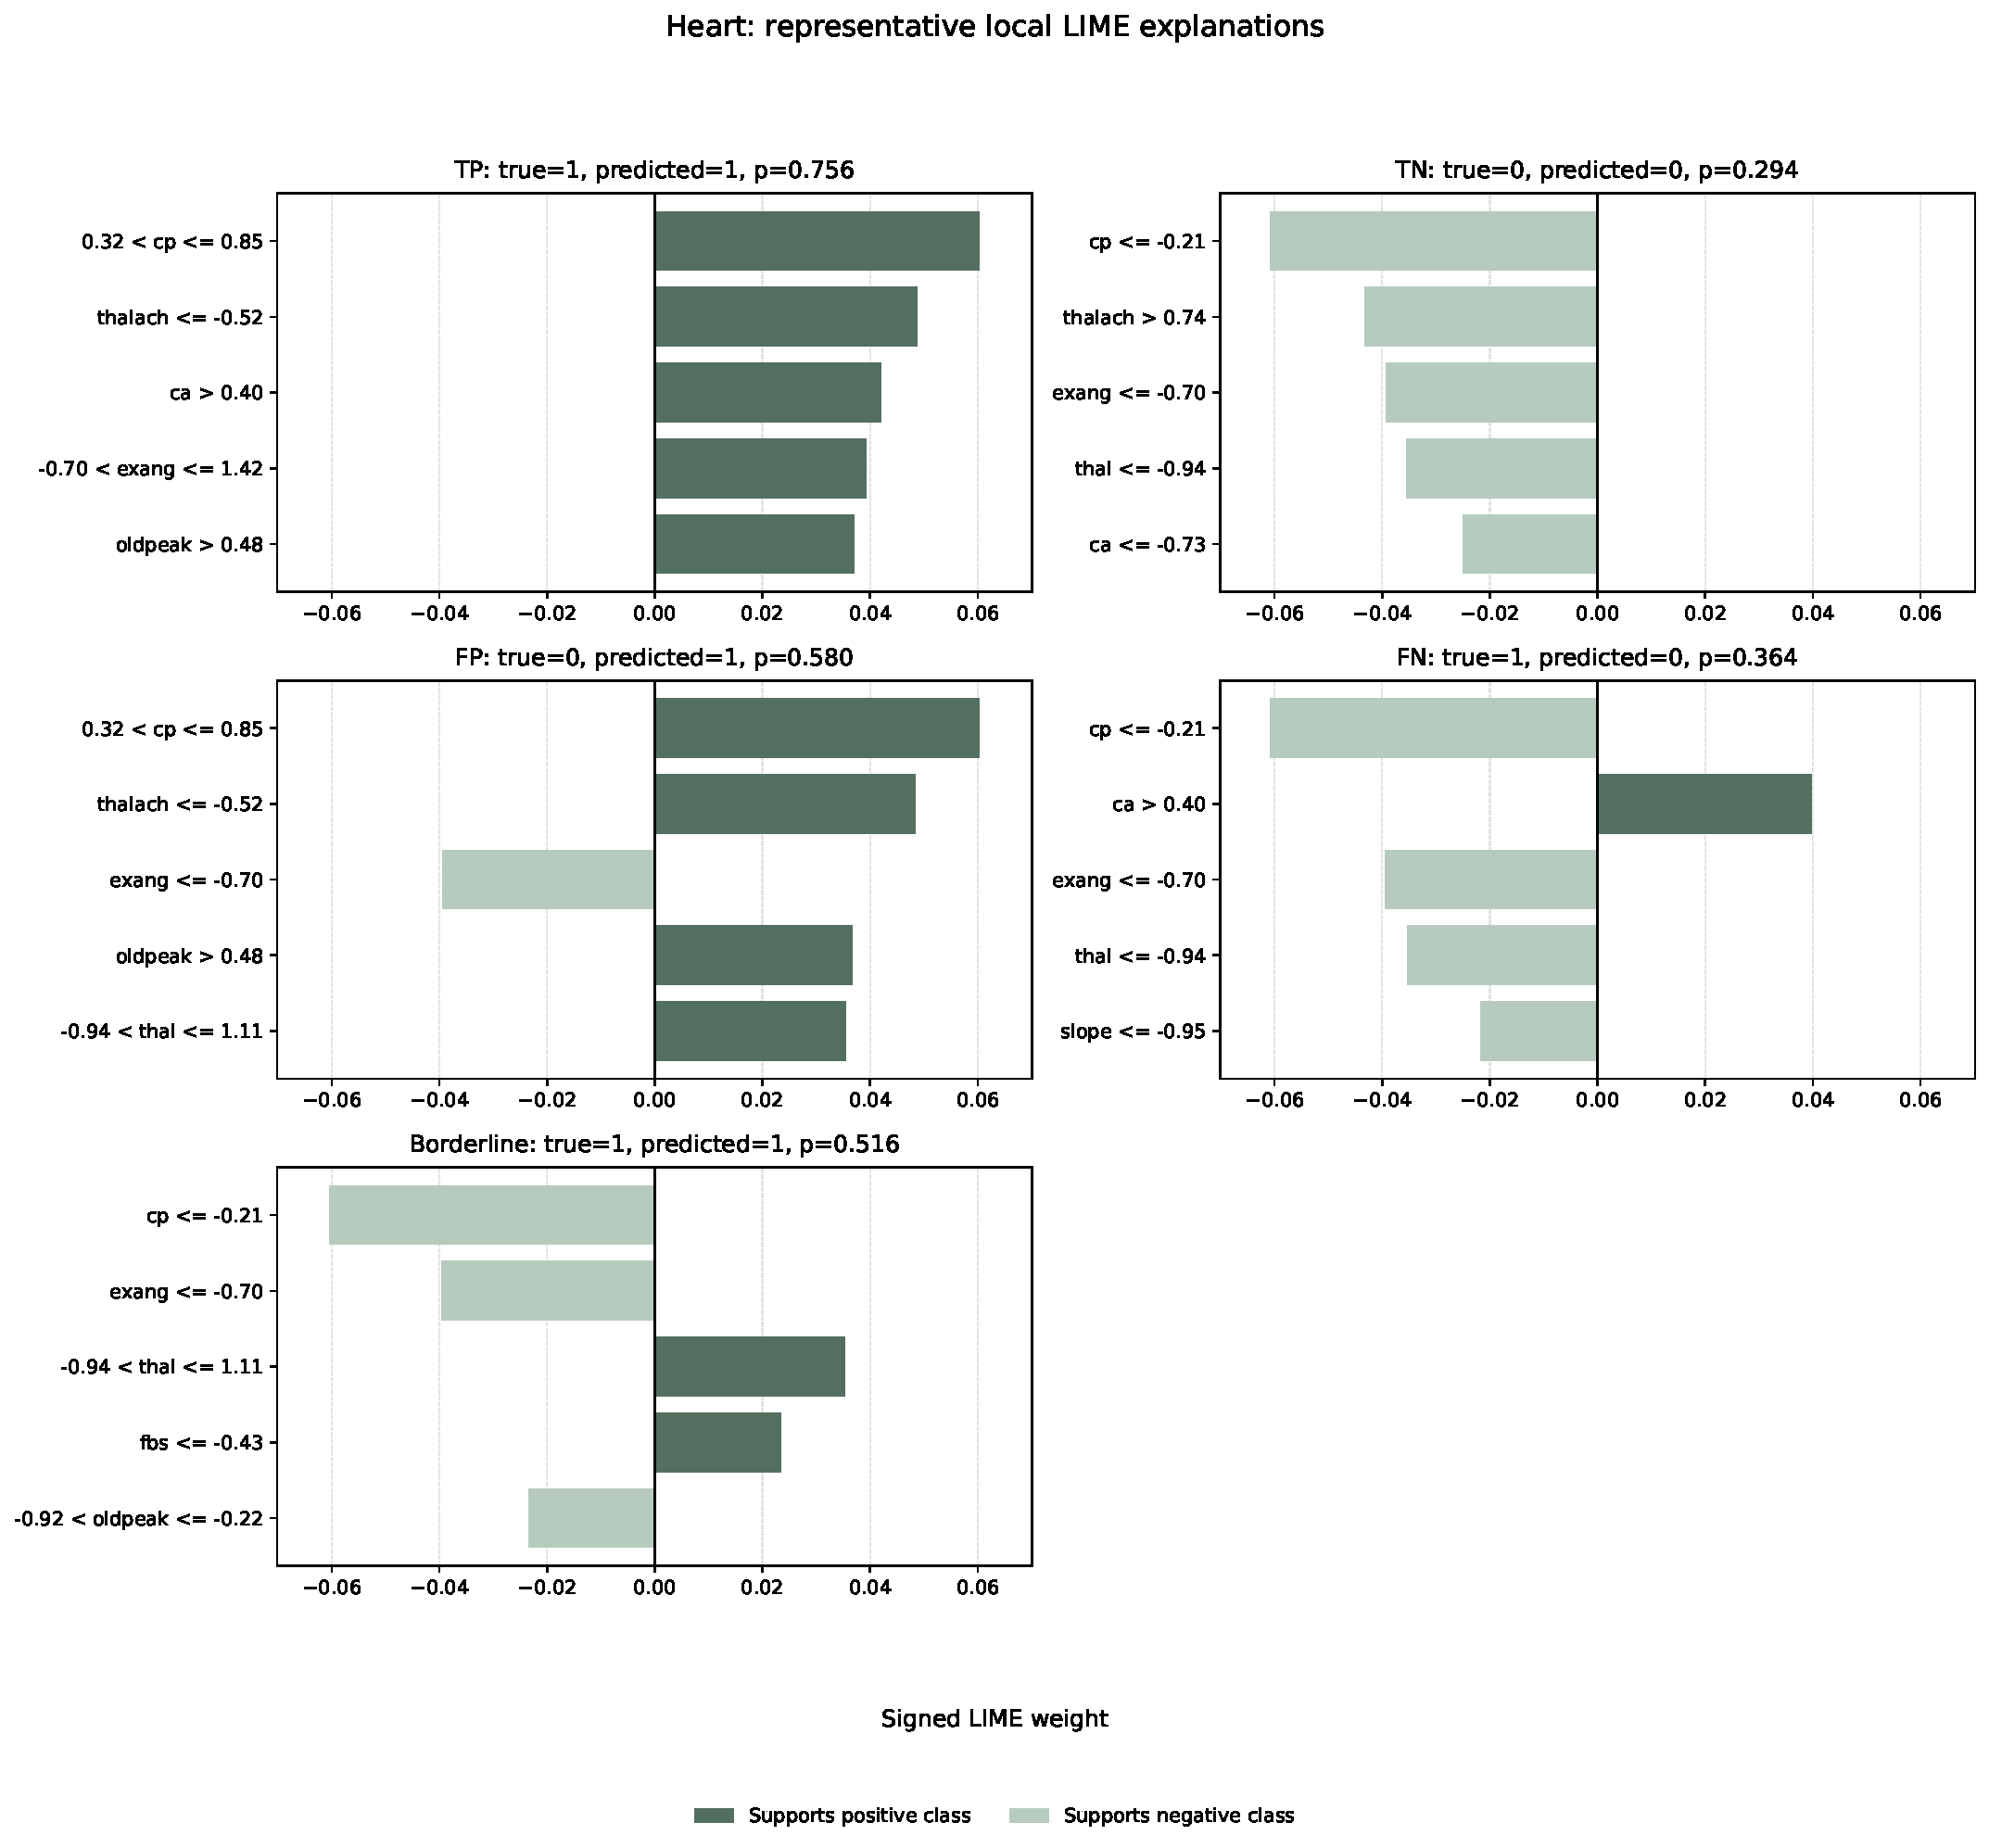
\includegraphics[width=0.95\textheight]{images/results/representative_lime_heart.pdf}
    \caption{Representative Heart \gls{lime} explanations for the available outcome categories. Rules were aggregated over the prespecified perturbation seeds.}
    \label{fig:representative_lime_heart}
\end{sidewaysfigure}

\begin{sidewaysfigure}[p]
    \centering
    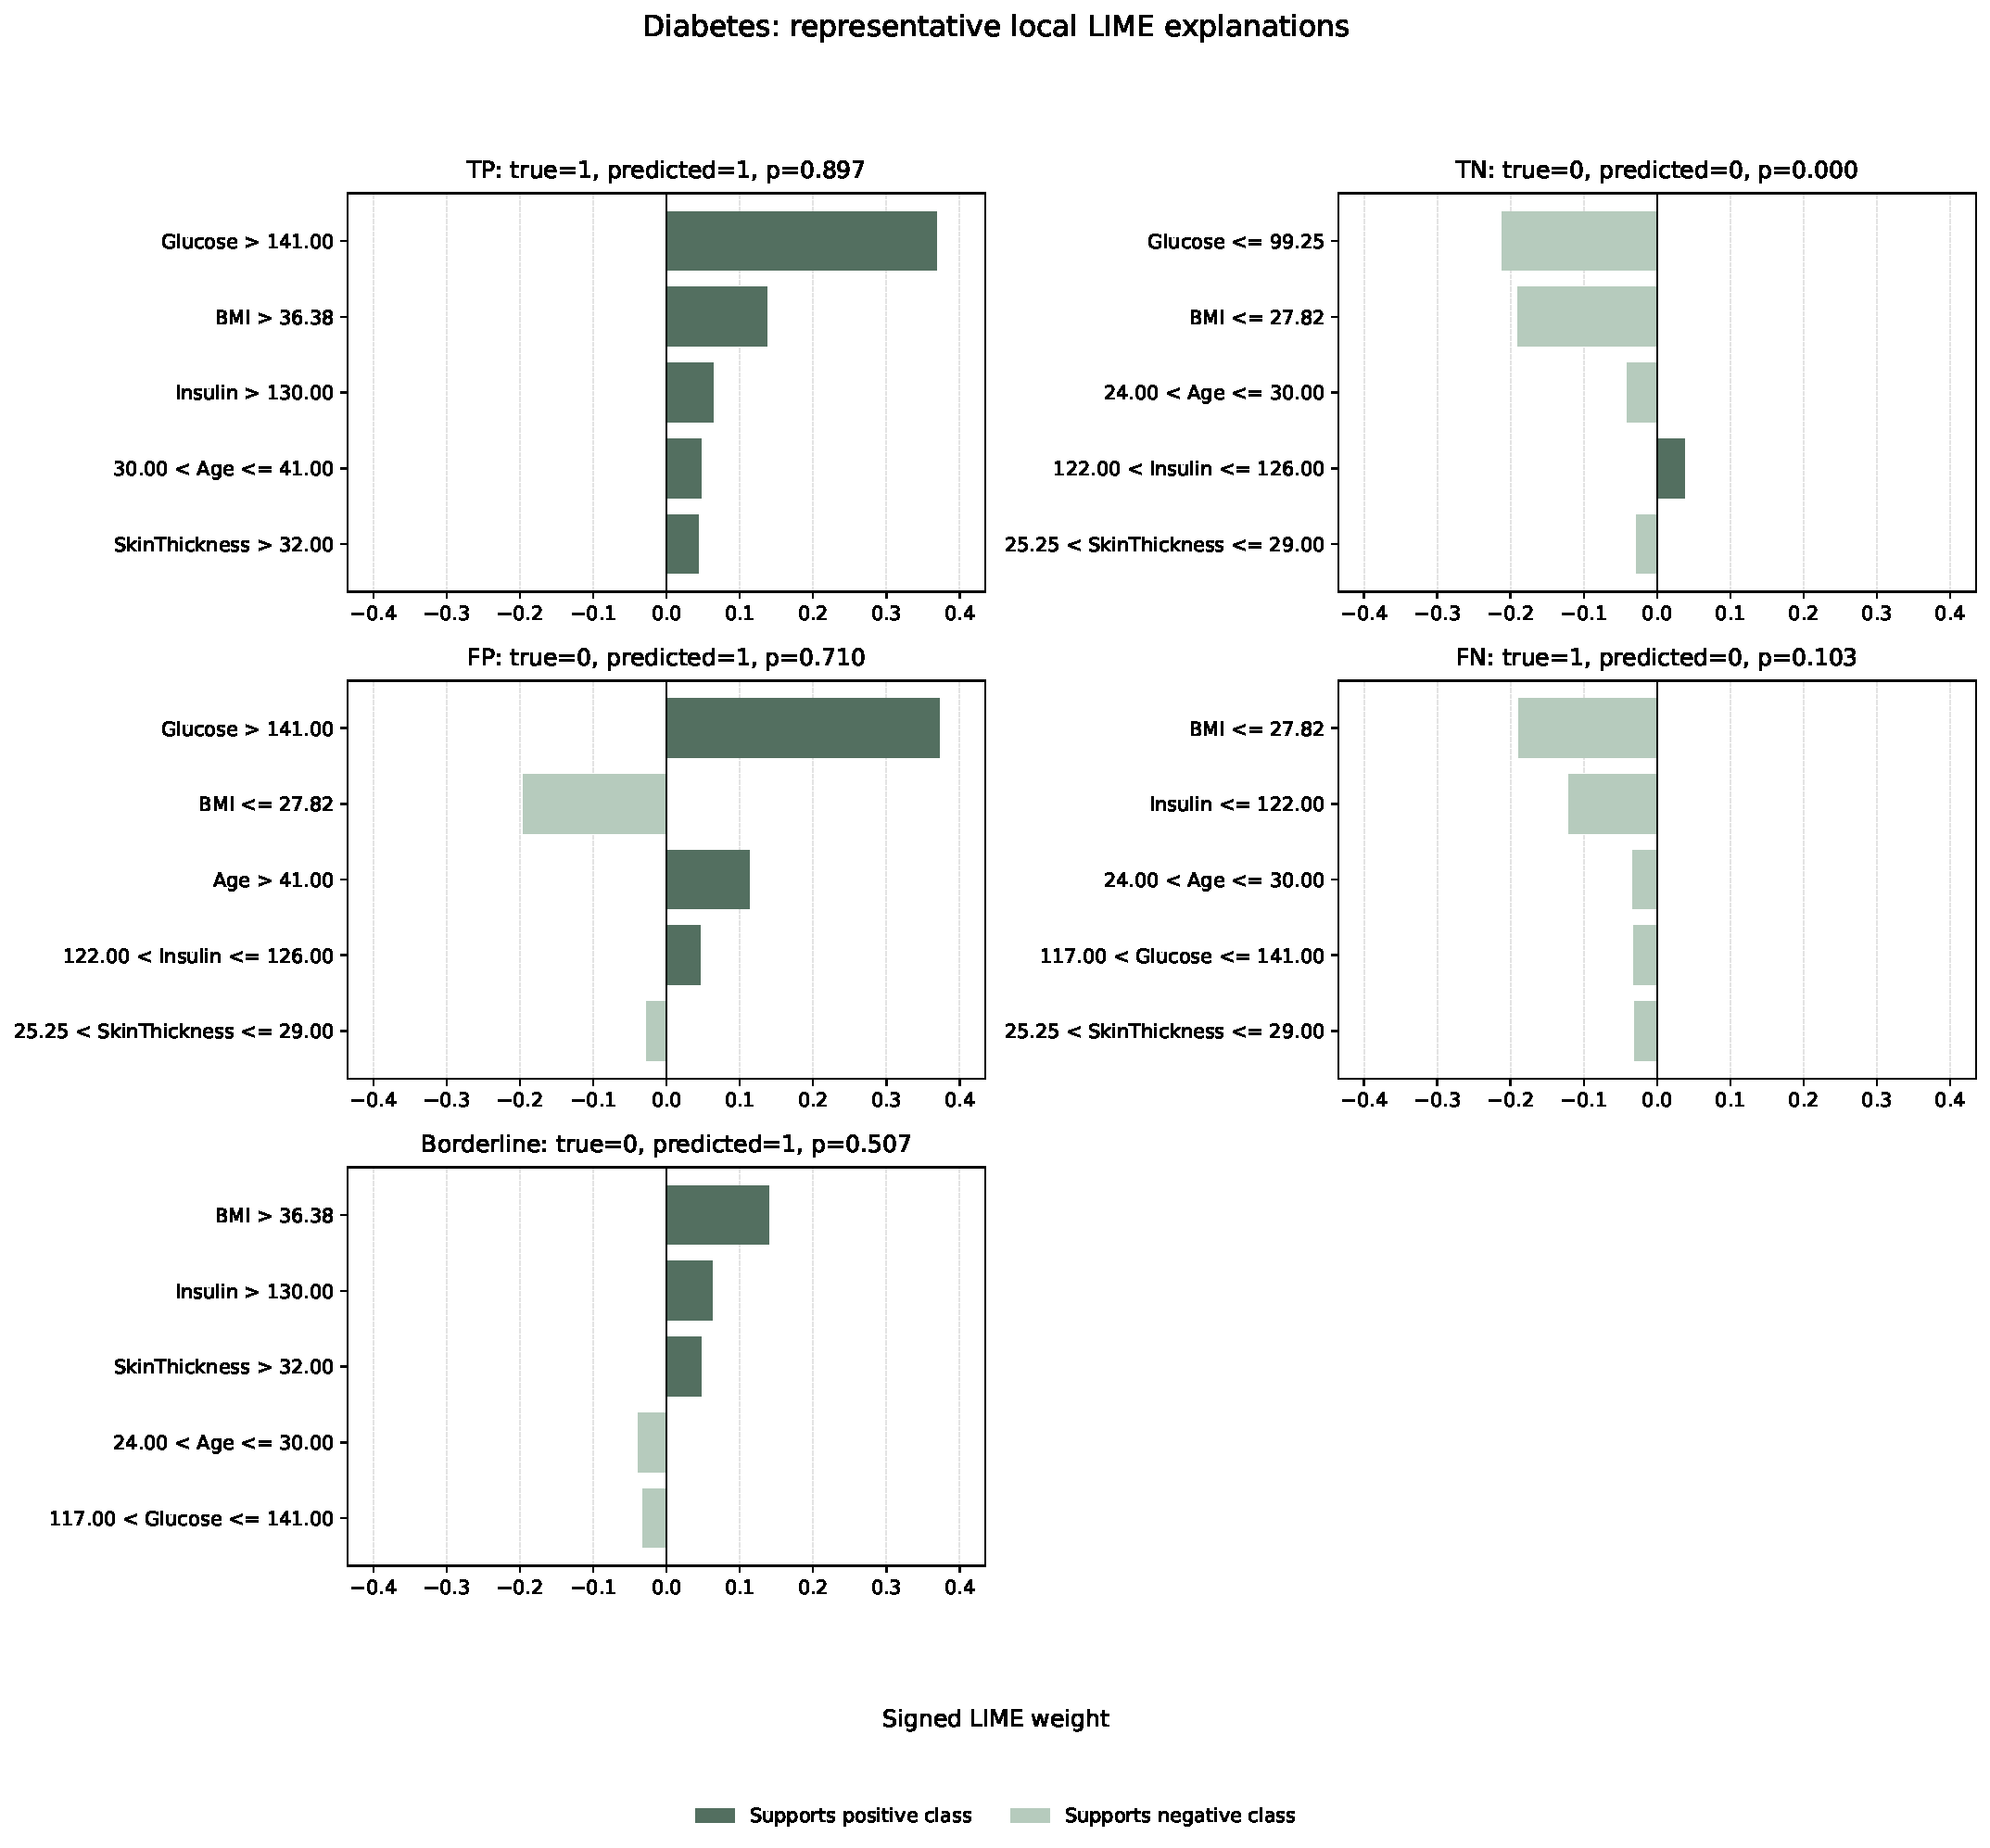
\includegraphics[width=0.95\textheight]{images/results/representative_lime_diabetes.pdf}
    \caption{Representative Diabetes \gls{lime} explanations for the available outcome categories. Rules were aggregated over the prespecified perturbation seeds.}
    \label{fig:representative_lime_diabetes}
\end{sidewaysfigure}

\begin{sidewaysfigure}[p]
    \centering
    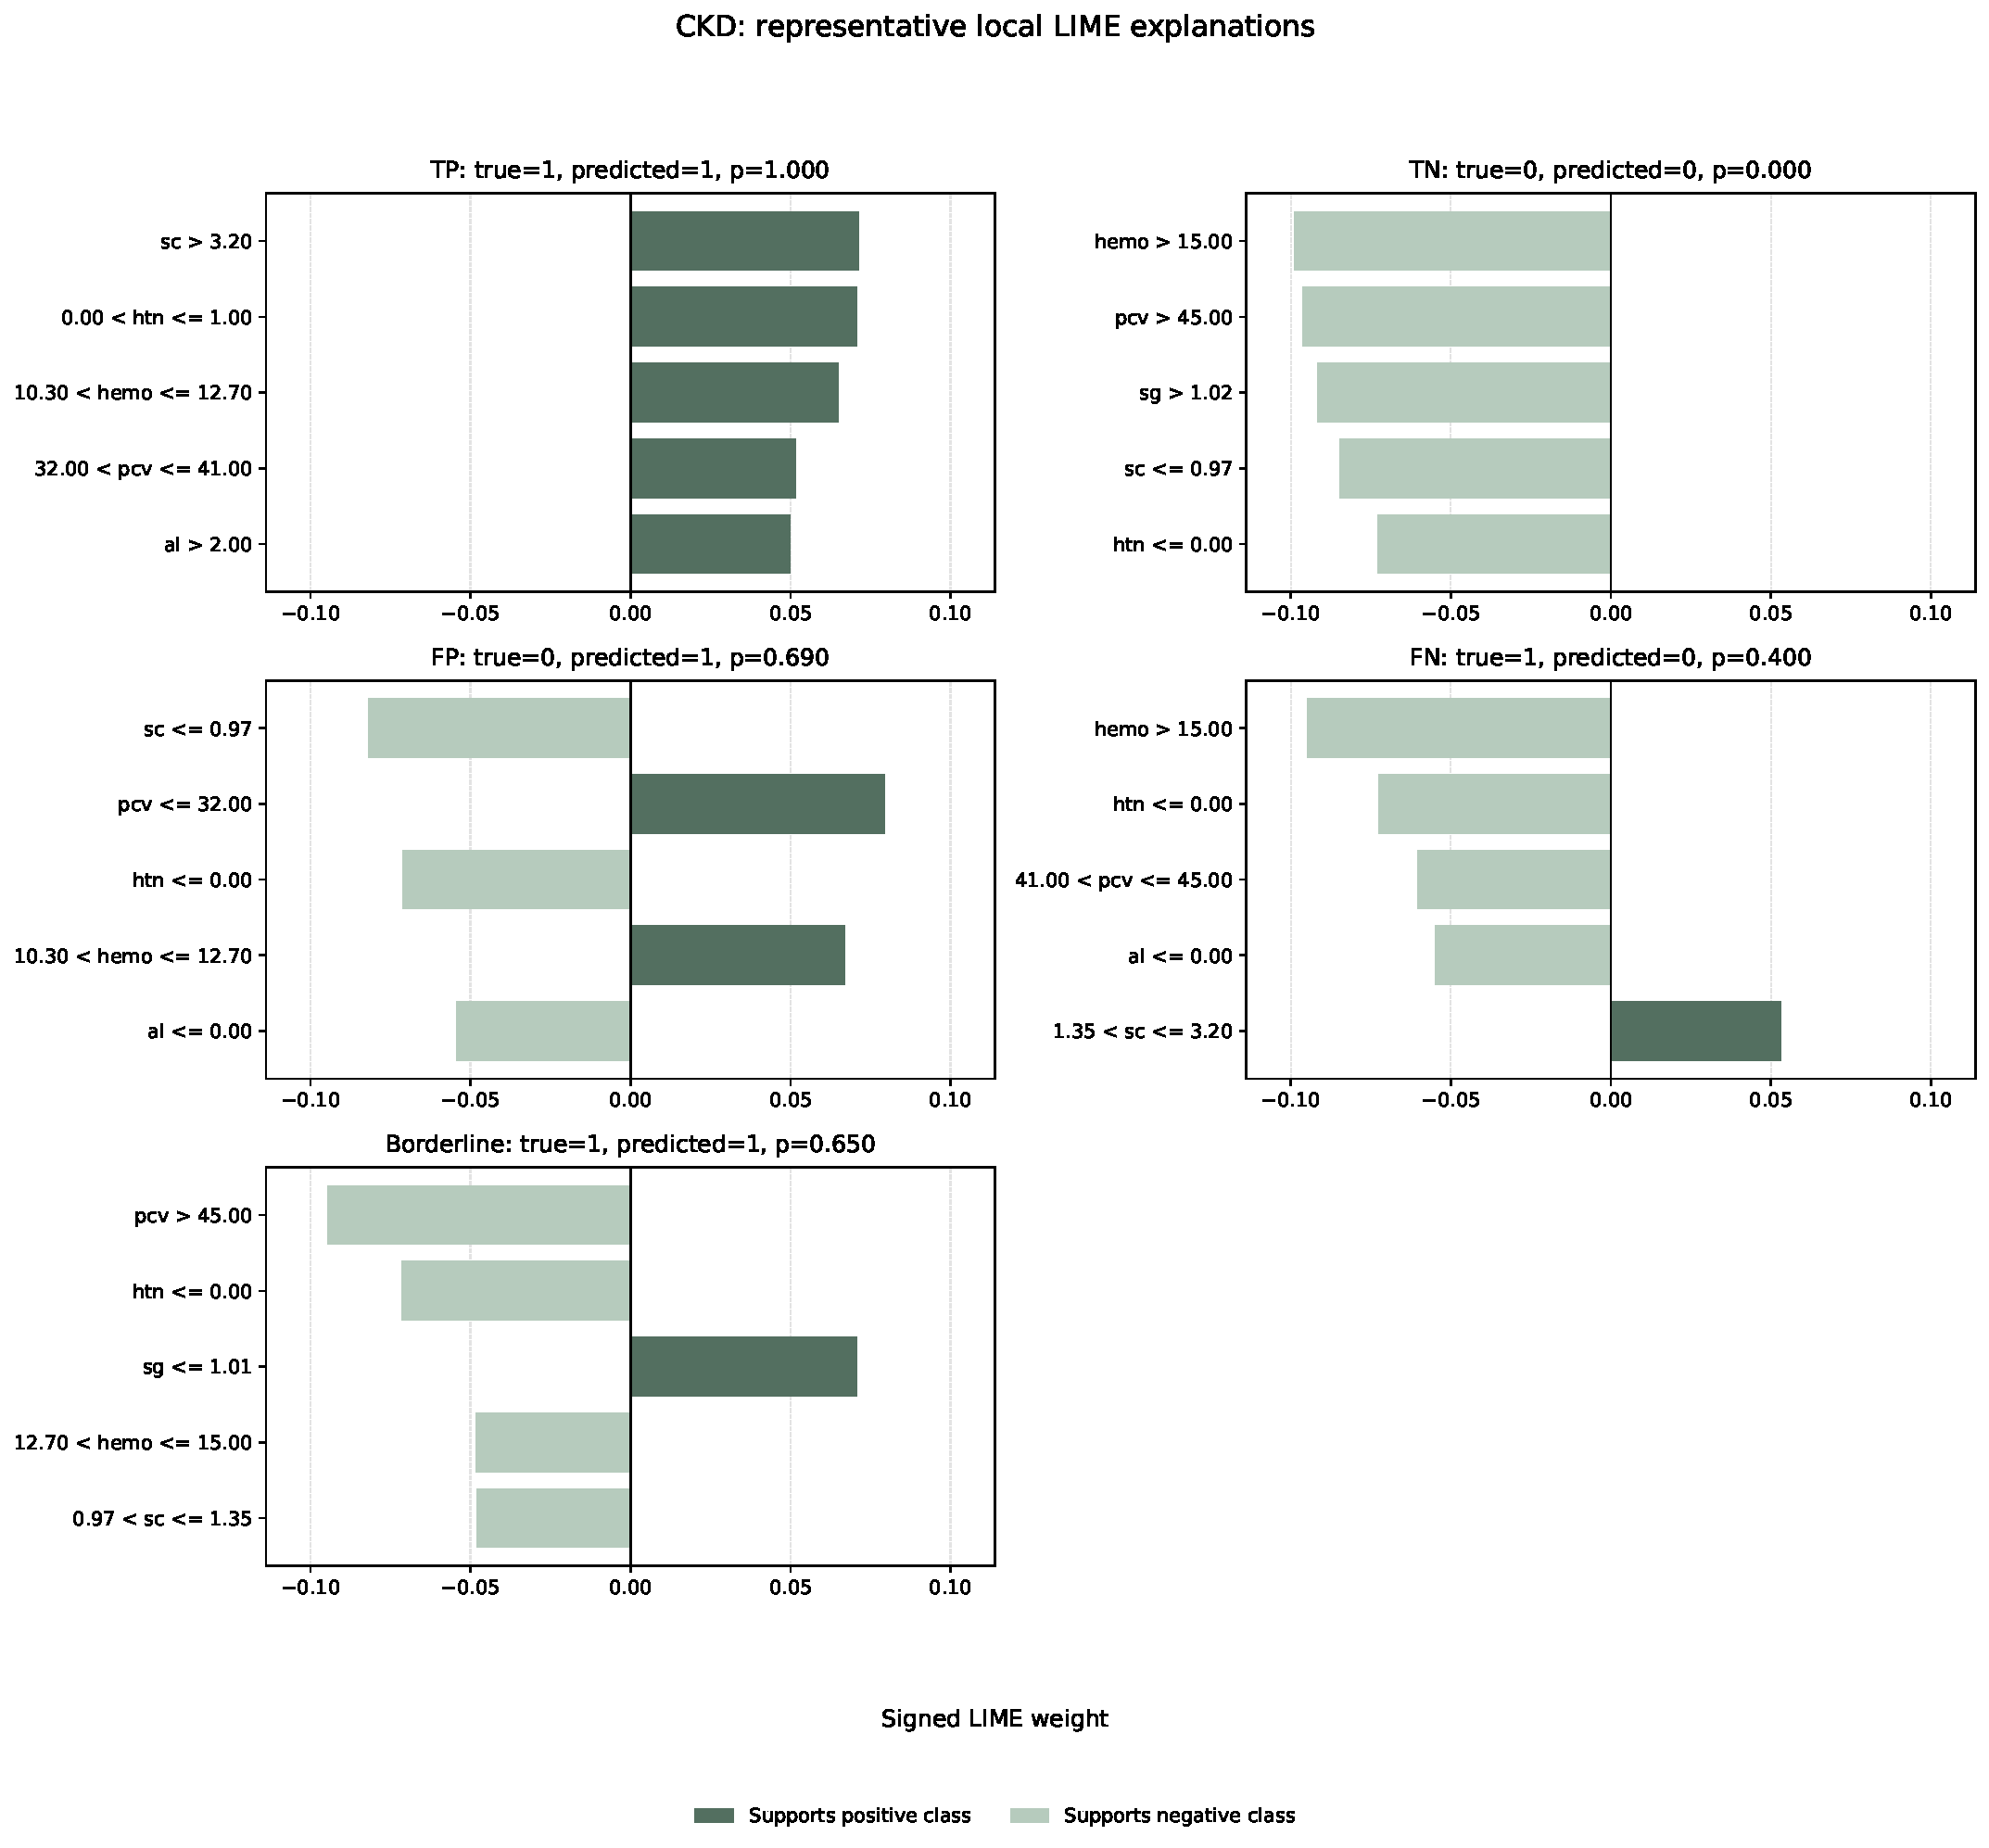
\includegraphics[width=0.95\textheight]{images/results/representative_lime_ckd.pdf}
    \caption{Representative \gls{ckd} \gls{lime} explanations for the available outcome categories. The held-out predictions contained only one false positive and one false negative.}
    \label{fig:representative_lime_ckd}
\end{sidewaysfigure}

\begin{sidewaysfigure}[p]
    \centering
    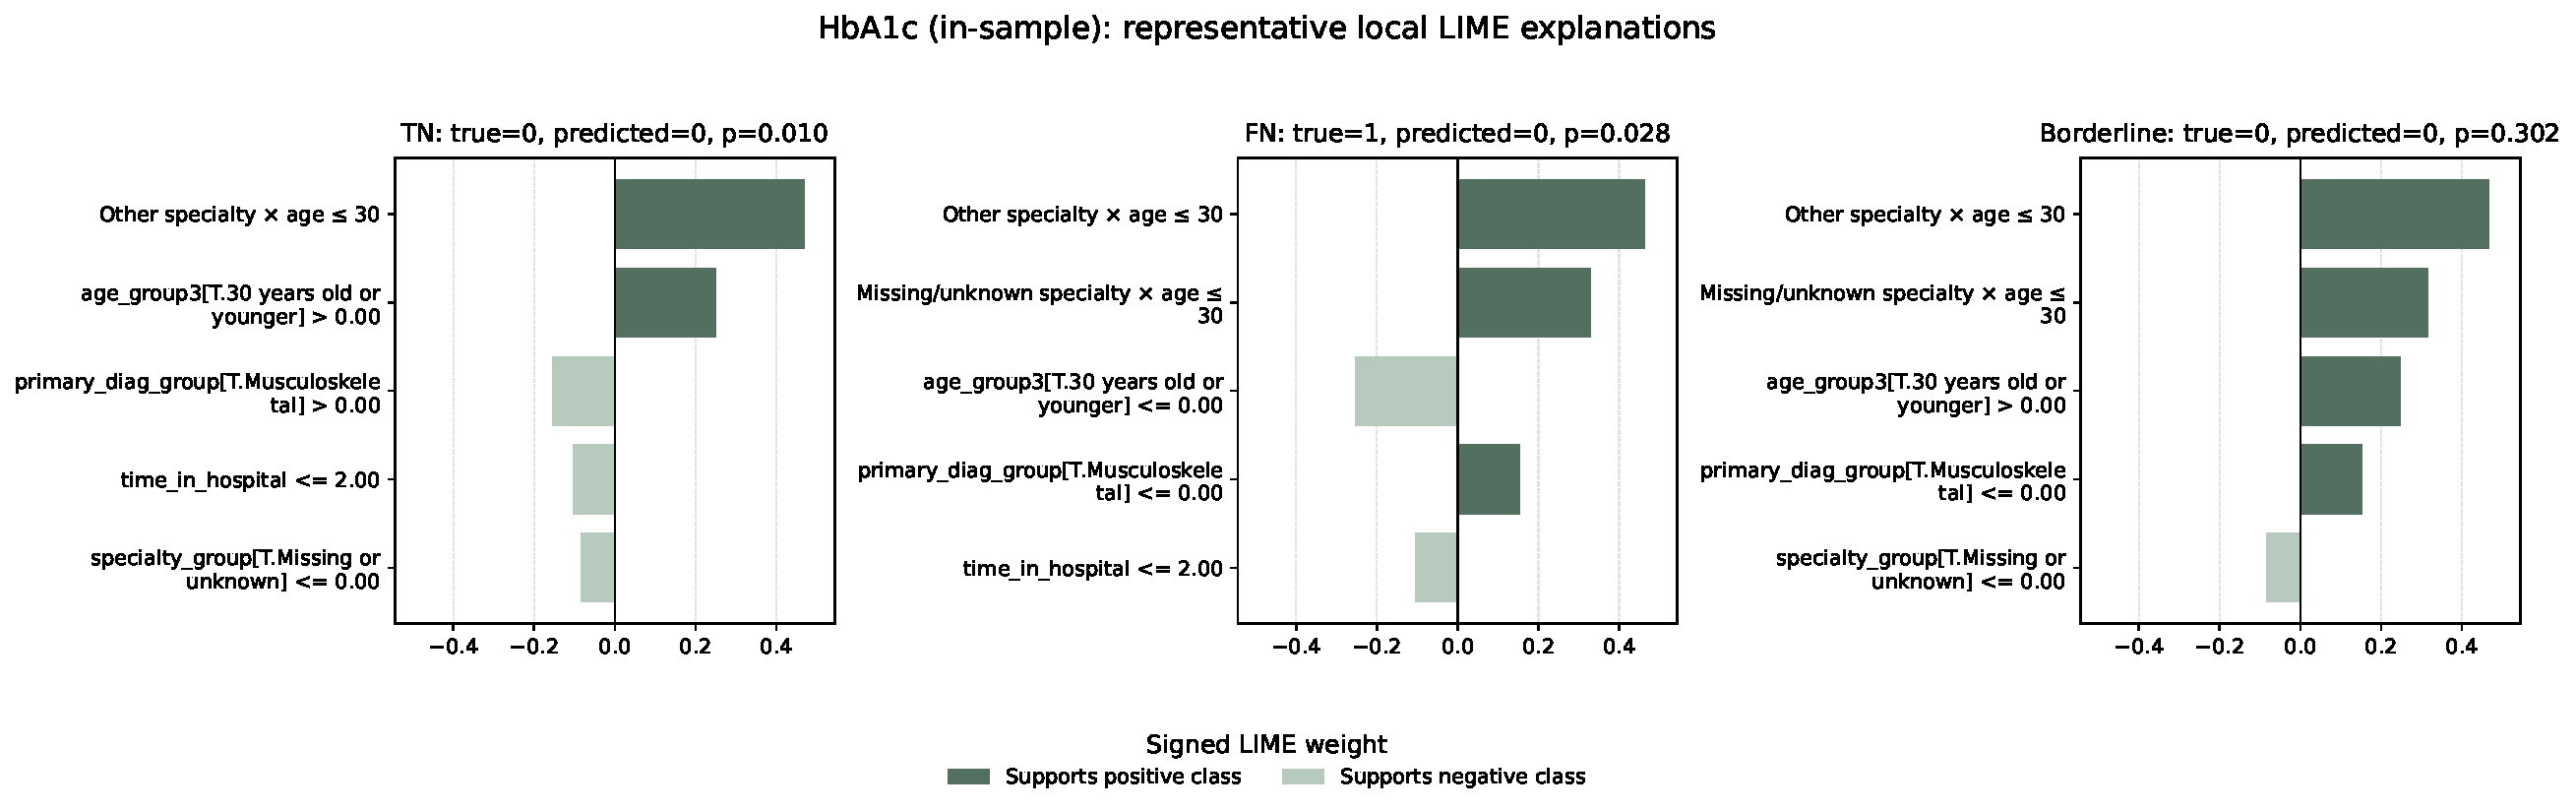
\includegraphics[width=0.95\textheight]{images/results/representative_lime_hba1c.pdf}
    \caption{Representative \gls{hbaone} \gls{lime} explanations for the available outcome categories. No positive classification was produced at the fixed threshold of 0.5.}
    \label{fig:representative_lime_hba1c}
\end{sidewaysfigure}